% !TEX root=/home/tavant/these/manuscript/src/manuscript.tex
\FloatBarrier
\section{Comparison of the \acs{DR} with the \acs{PIC} simulations}
  \label{sec-DR-results}
  
  In this section, we continue to analyze the simulation results described in \Cref{sec-PIC-ECDI}.
  First, we described in \cref{subsec-VDFpic} the velocity distribution functions (VDF) measured in the simulation.
  Then, we solve the relation dispersion with the measured VDFs, for both the \ac{ECDI} (\cref{eq-drECDI}) and the \ac{IAW} waves (\cref{eq-drIAWgene}), with the solved developed in \Cref{sec-DR-solver}.

  \subsection{Temporal evolution of the distribution functions in the \acs{PIC} simulation} \label{subsec-VDFpic}
  
  To begin with, we visualize and comment the distribution functions measured in the \ac{PIC} simulation.
  \Cref{fig-vdfs_pic_time} shows at different times in the simulation the normalized electron azimuthal velocity distribution functions (the ion VDF is showed in \cref{fig-ivdfs_pic_time}).
  The velocities are normalized by the electron thermal velocity.
  To help reading the figure, the  theoretical electron drift velocity $u_e = \frac{E_z}{B_r}$, normalized to the electron thermal velocity is shown.
  The distributions are averaged in time over $4\,\nano\second$, and in space over all the azimuthal direction and over a small length in the radial direction at the center of the channel, between $r=0.45\,\centi\meter$ and $r=0.55\,\centi\meter$.
  
  \begin{figure}[!hbt]
    \centering
    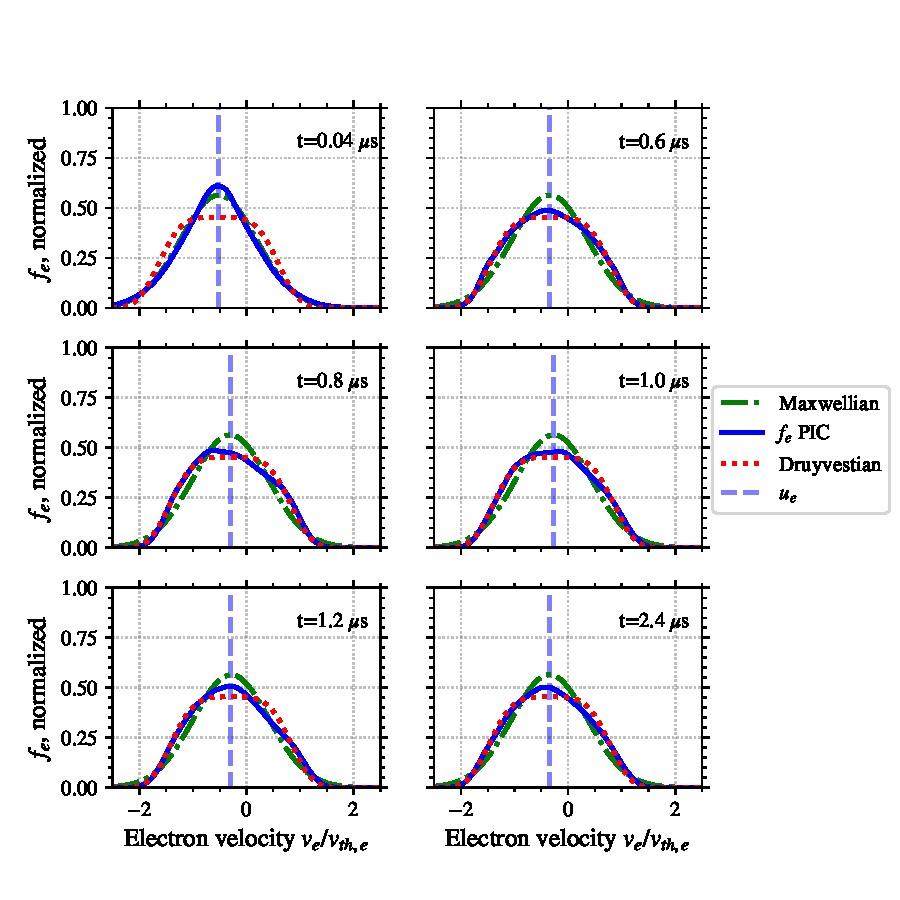
\includegraphics[width=0.95\textwidth]{Distributions_time_evolution_evdf.pdf}
    \caption{(solid blue) Electron normalized azimuthal velocity distribution functions at different times of the simulation. The velocity is normalized by the electron thermal velocity; (dashed light blue) The theoretical $E\times B$ drift velocity of the electrons $u_e = \frac{E_z}{B_r}$; (dotted-dashed green) Maxwellian  distribution function with the same density, mean velocity and temperature as the measured \acs{EVDF}.}
    \label{fig-vdfs_pic_time}
  \end{figure}
  
  We can see in \cref{fig-vdfs_pic_time} that the electron mean velocity is always near the $E \times B$ drift velocity, which is of the order of one quarter of the electron thermal speed.
  The shape of the distribution functions is slightly different from the Maxwellian distribution, with smaller maximum and a wider distribution, similarly to a Druyvesteyn distribution.
  
  \Cref{fig-ivdfs_pic_time} shows at different times in the simulation the normalized ion azimuthal velocity distribution functions.
  As in \cref{fig-vdfs_pic_time}, the mean velocity is shows, and a Maxwellian distribution of same density, mean velocity and temperature is shown.


  
  \begin{figure}[!hbt]
    \centering
    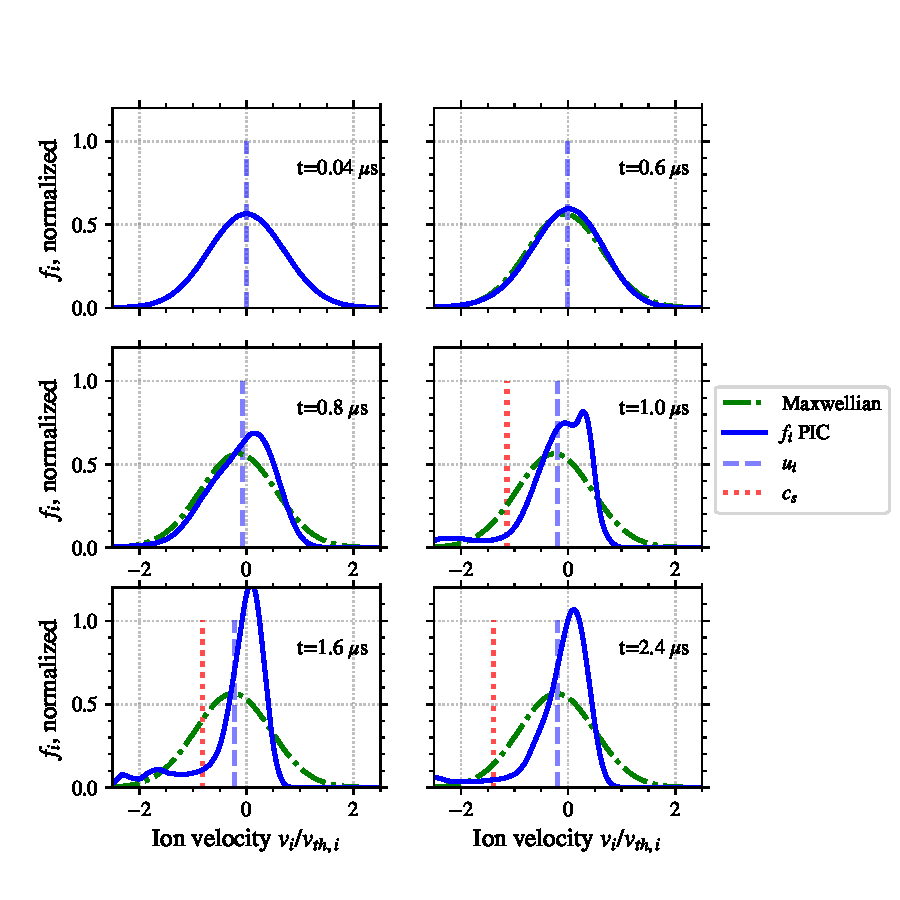
\includegraphics[width=0.95\textwidth]{Distributions_time_evolution_ivdf.pdf}
    \caption{Electron and ion normalized azimuthal velocity distribution functions at different times of the simulation. The velocity is normalized by the thermal speed of the corresponding species. The theoretical $E\times B$ drift velocity of the electrons $u_e = \frac{E_z}{B_r}$, and the ion sound speed $c_s$ normalized by the ion thermal velocity are also displayed.}
    \label{fig-ivdfs_pic_time}
  \end{figure}
  
  At the beginning of the simulation the ions are Maxwellian with a zero mean velocity.
  Starting from $t=0.8\,\micro\second$, the ions are dragged in the same direction as the electron drift.
  This is characteristic of the ion-wave trapping \citep{lafleur2017a}.
  Consequently, the ion distribution function is significantly different from the Maxwellian.
  Indeed, because of the particle-wave interactions a small population of high energy ions is generated. 
  This leads to both an increase of the ion temperature, and the formation of a drift velocity in the azimuthal direction.
  The high energy ion population comes from ion-wave trapping, as we can see that their velocity is of the order of the ion sound speed, which is close to the wave phase velocity \citep{lafleur2018}.
  We can see that the trapped population is larger at $t=1.6\,\micro\second$ compared to $t=2.44\,\micro\second$.
  This is consistent with the discussion of \cref{subsec-temp}, as we can see in \cref{fig-oscillation_ion_cret} that at $t=1.4\,\micro\second$  the ion temperature is large, and the wave energy density $\epsilon_{\rm wave}$ is large compared to the thermal energy density $\epsilon_{\rm th}$, while at $t=2.4\,\micro\second$ the ion temperature is small and we have $432\epsilon_{\rm wave} \simeq \epsilon_{\rm th}$.
  
  As both electron and ion velocity distribution functions are different from a drifting Maxwellian, we will study the influence of both distributions in the calculations of the dispersion relation.
  
  
  \FloatBarrier
  \subsection{Resolution of the electron cyclotron drift instability} \label{subsec-ECDIPIC}
  
    As observed in \Cref{sec-PIC-ECDI}, the simulation begins with a linear growth of the instability.
    Previous results obtained with \LPPic \citep{croes2017a} showed no cyclotron resonances (also known as Bernstein resonances) during this period.
    However, these results were obtained with Lafleur's convection model, as introduced in \cref{sec-reinjectionnoise}.
    Here, the results were obtained with the modified model, inducing less noise.
    
    We can see in \Cref{fig-phi_fluctuation_summary}  a snapshot of the plasma potential fluctuation in the azimuthal direction \[ \delta \phi(r, \theta) = \phi(r, \theta) - < \phi(r, \theta) >_{ \theta}, \]
    at four different times during the growth of the instability.
    For these results, we increased the azimuthal length $L_{\theta}$ from $2.5$ to $6.2\,\milli\meter$ compared to the simulations of \cref{sec-PIC-ECDI}, so that the instability characteristics, as the wavenumber $k_{\theta}$, are better resolved.
    We observe no significant differences on the simulation results.
    However, the simulation time is doubled in this case, so only the first microsecond have been simulated.
    
    \begin{figure}[!hbt]
      \centering
      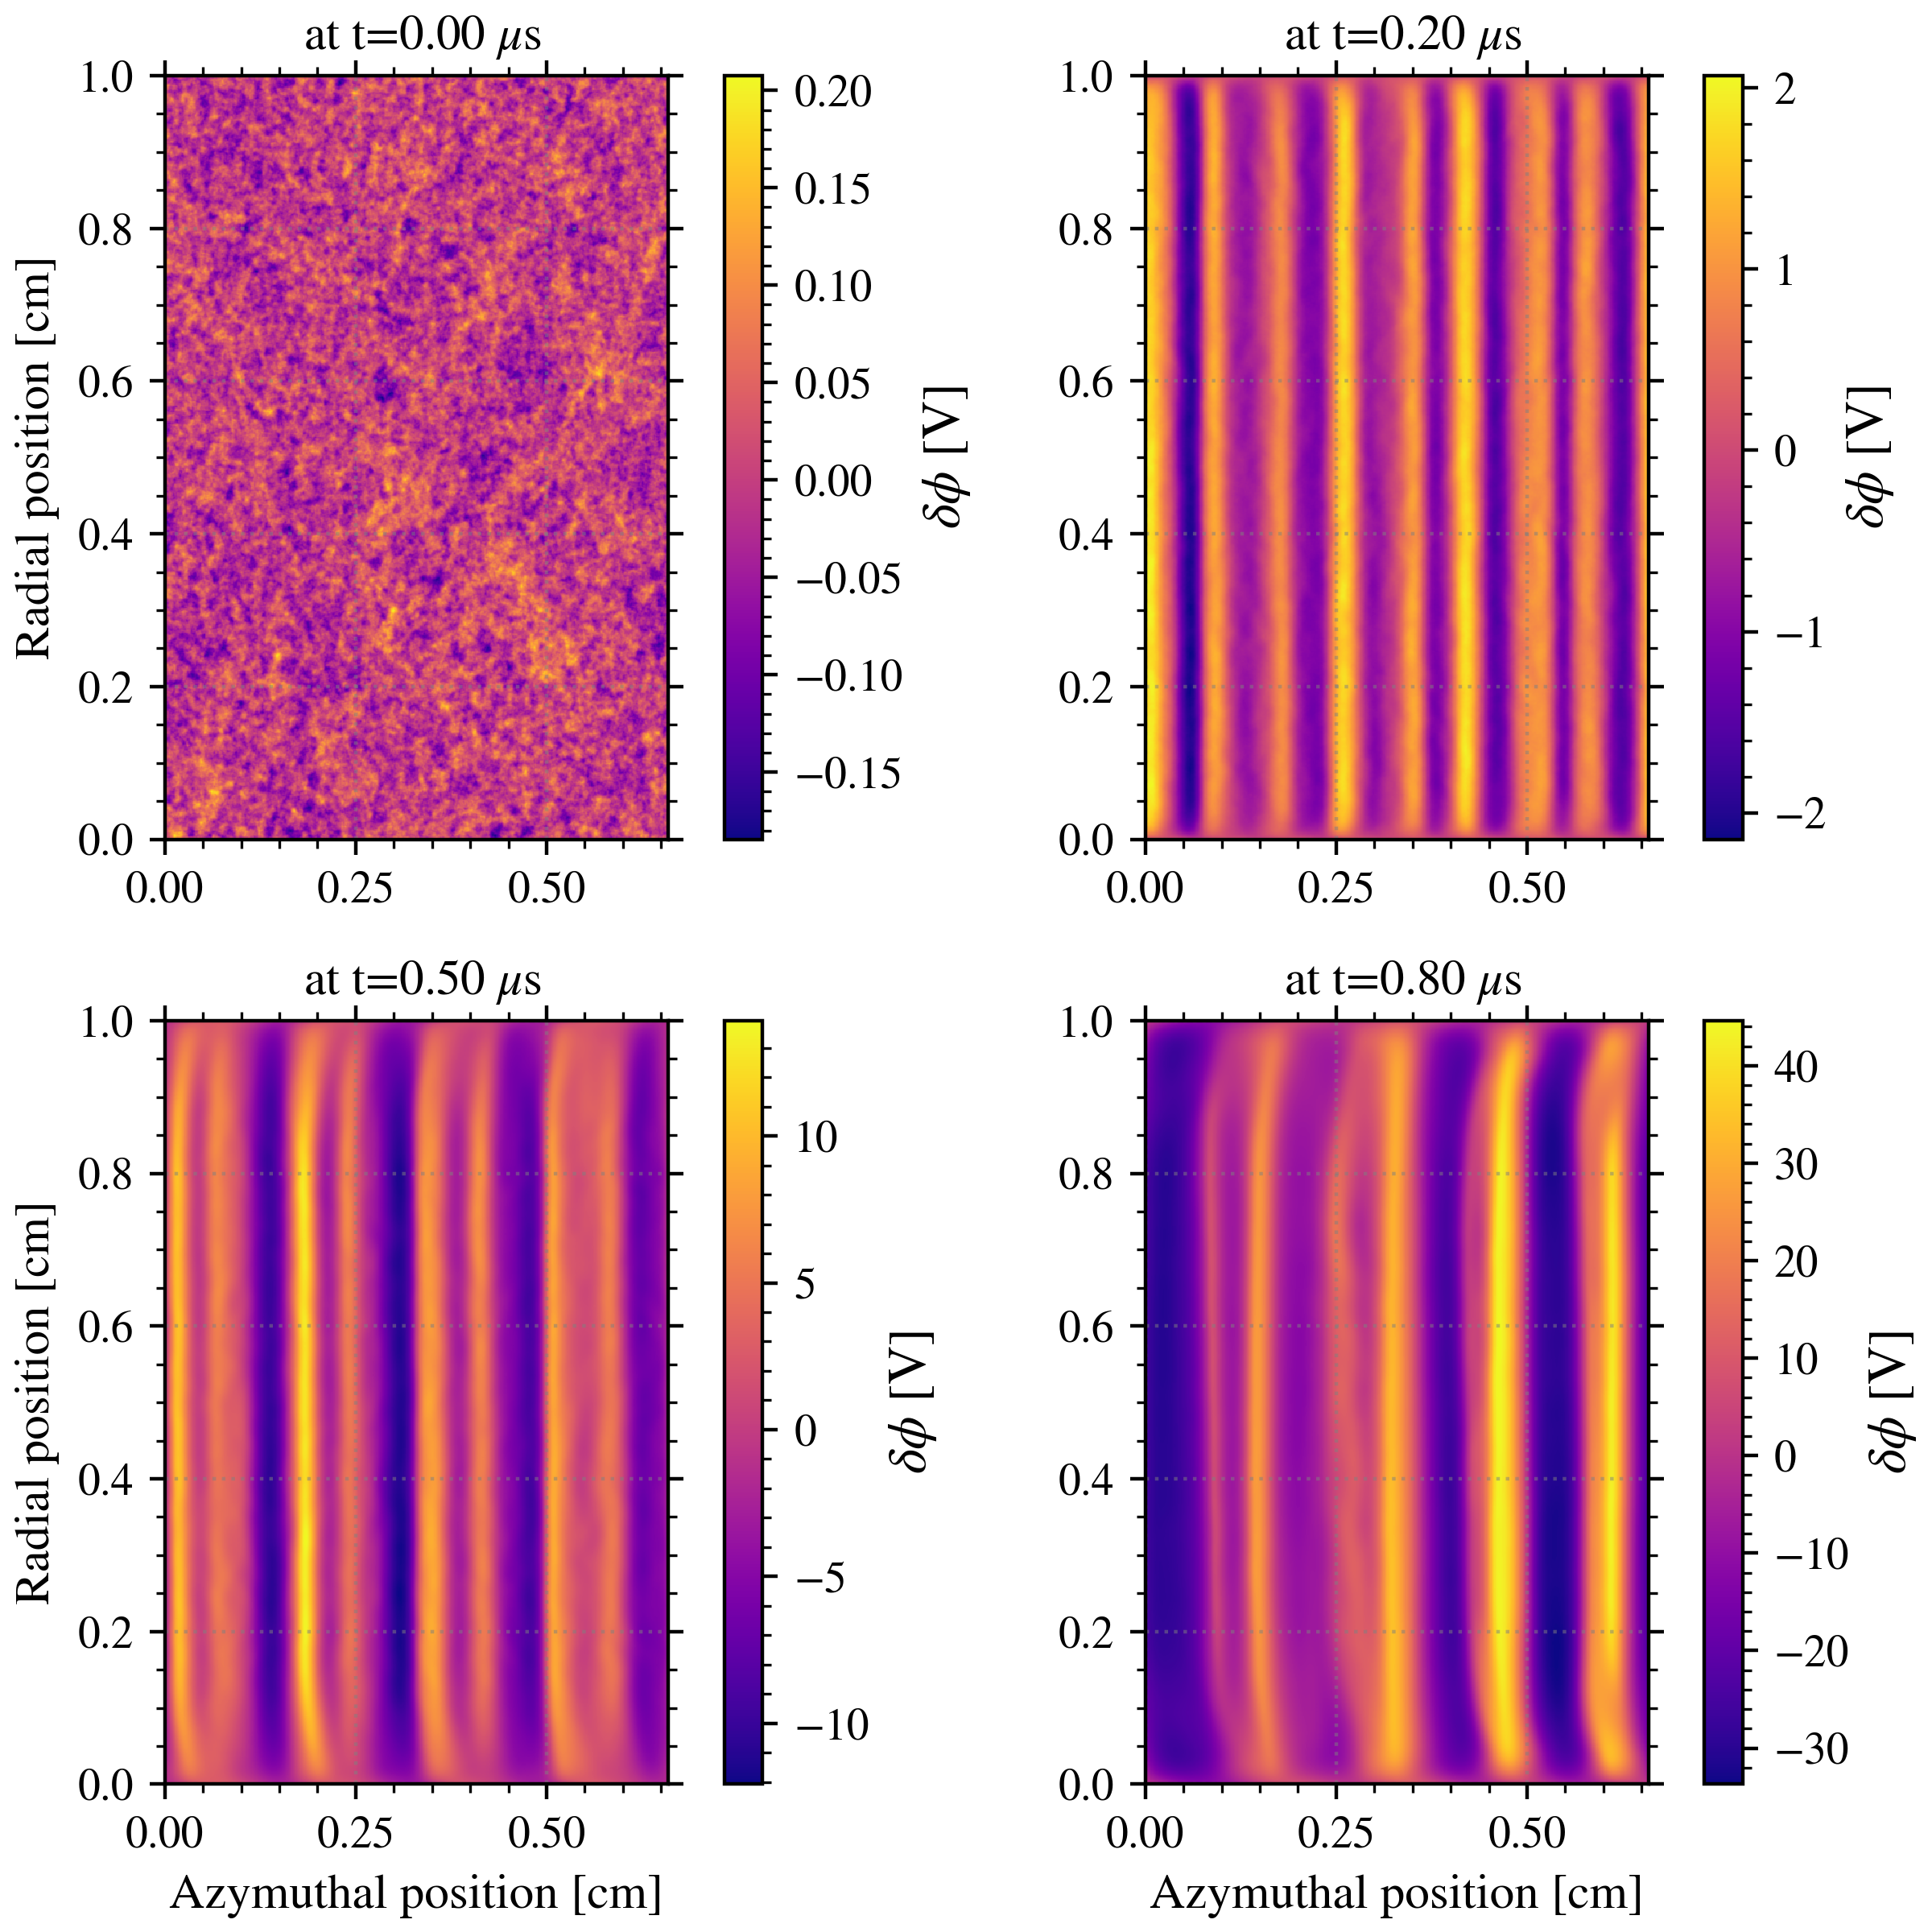
\includegraphics[width=0.9\textwidth]{phi_fluctuation_summary.png}
      \caption{Radial-azimuthal distribution of the oscillation of the plasma potential $\delta \phi(r, \theta) = \phi(r, \theta) - < \phi(r, \theta) >_{ \theta}$ at different times during the linear phase of the simulation using an increased azimuthal length. The frequency spectra of each snapshot is shown in \cref{fig-phi_fluctuation_summary_FFT}. }
      \label{fig-phi_fluctuation_summary}
    \end{figure}
    
    At the beginning, we see fluctuations that can be due to both thermal fluctuation \citep{salpeter1960} or numerical noise due to particle discretization.
    Then, the instability rises.
    We can see that it starts with small wavelength ($\lambda \simeq 0.75\,\milli\meter$ at $t=0.2\,\micro\second$).
    After a short period, the short wavelength waves merge to form longer wavelength waves  ($\lambda \simeq 1.5\,\milli\meter$ at $t=0.7\,\micro\second$).
    
    \begin{figure}[!hbt]
      \centering
      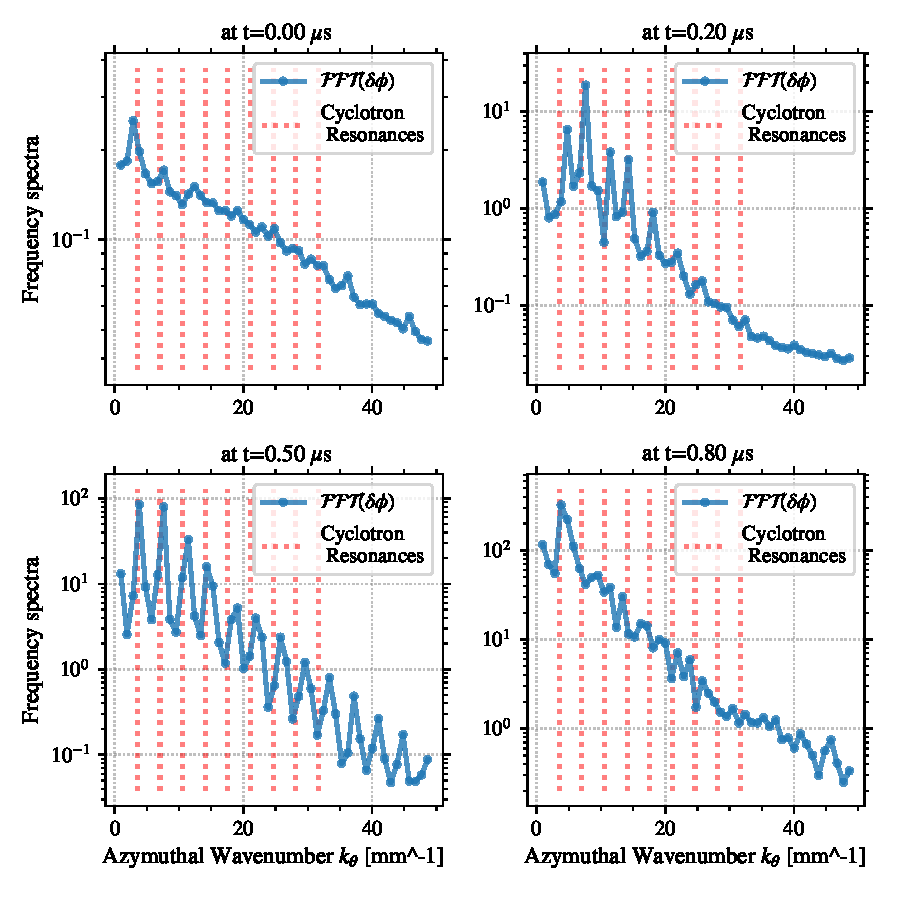
\includegraphics[width=0.8\textwidth]{phi_fluctuation_summary_FFT.pdf}
      \caption{Frequency spectra on the azimuthal instability presented in \cref{fig-phi_fluctuation_summary}. Each spectrum is averaged in the radial direction. The red dotted lines represent the cyclotron resonances $k_{\theta} = n \dfrac{\oce}{u_e}$ with $n \in \mathbb{N}$.}
      \label{fig-phi_fluctuation_summary_FFT}
    \end{figure}
    
    The evolution of the instability is also clearly seen on the frequency spectra, showed in \Cref{fig-phi_fluctuation_summary_FFT}.
    The spectra are obtained with the FFT algorithm, and are averaged in the radial direction.
    We can see in the spectra the resonances at multiple of the cyclotron wavenumber $k_0 = \frac{\oce}{u_e} \simeq 3.5\,\milli\meter^{-1}$.
    At $t=0.2\,\micro\second$, the most dominant mode is the second resonance, but the other resonances are also present.
    At $t=0.5\,\micro\second$, all the resonances are distinguishable, but their amplitude is strictly decreasing.
    Then, at $t=0.8\,\micro\second$, we can no longer see the resonances, except for the first one.
    % As we observed during the first stages of the simulation the resonances in the Fourier spectrum, we solve the dispersion relation for the \ac{ECDI}.
    
    \vspace{1em}
    We now solve the \ac{ECDI} dispersion relation of \cref{eq-drECDI} for $t=0.2, 0.4$ and $0.7\micro\second$ using both the Maxwellian hypothesis for the ions and electrons, and the velocity distribution functions measured in the \ac{PIC} simulations.
    The radial wavenumber taken is $k_r = 2 \pi/L_R \sim 0.6 \per\milli\meter$ \citep{lafleur2016,janhunen2018}.
    This value corresponds to $k_r \lde = 0.036$ at $t=0.2\,\micro\second$ and $k_r \lde = 0.044$ at $t=0.7\,\micro\second$, as the electron temperature increases.

    \begin{figure}[!hbt]
      \centering
      % \begin{tabular}{@{} c}
        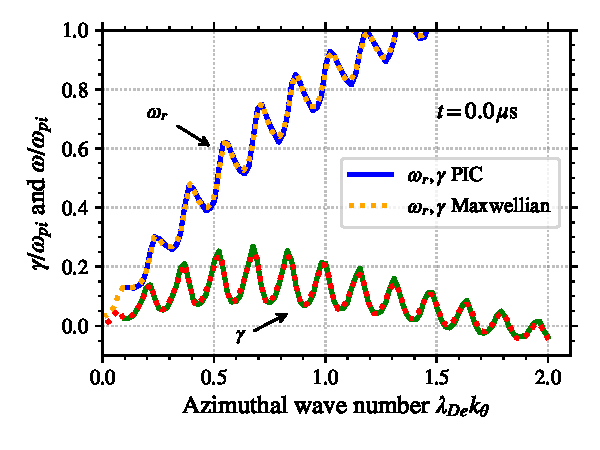
\includegraphics[width=0.49\textwidth]{ECDI_PIC_ionvcorrected_2mus.pdf} 
        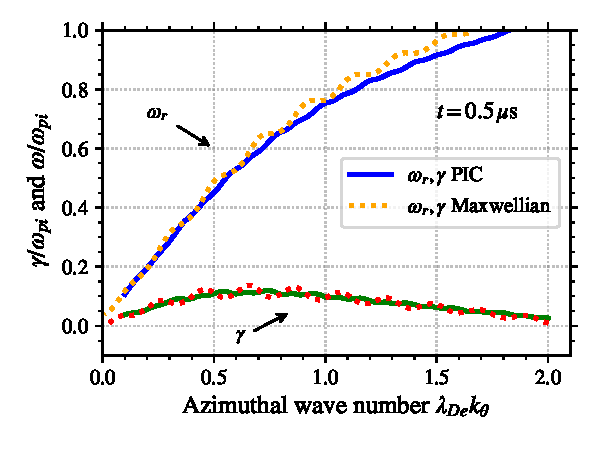
\includegraphics[width=0.49\textwidth]{ECDI_PIC_ionvcorrected_5mus.pdf} 
        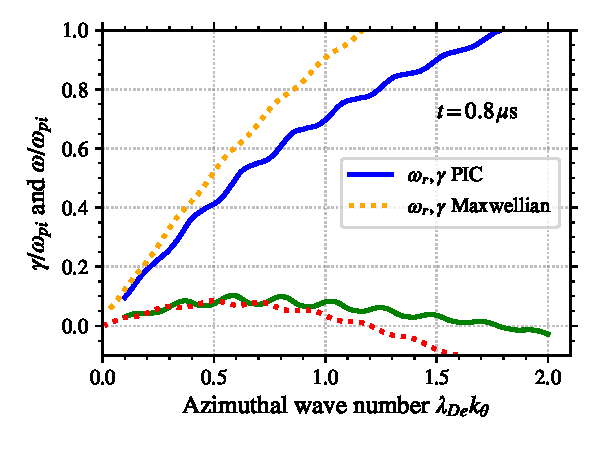
\includegraphics[width=0.49\textwidth]{ECDI_PIC_ionvcorrected_8mus.pdf} 
      % \end{tabular}
      \caption{Dispersion relation for the \acs{ECDI} using (dotted lines) the Maxwellian hypothesis for the ions and electrons, and (solid lines) the velocity distribution functions measured in the \acs{PIC} simulations. The wavenumber is normalized by the Debye length, and the pulsation and the growth rate are normalized to the ion pulsation frequency.}
      \label{fig-DRECDI}
    \end{figure}
    
    We can see in \Cref{fig-DRECDI} that the dispersion relation shows the cyclotron resonance at the beginning.
    However, the most growing wavelength is not the second harmonic, but the fourth.
    After $t=0.5\,\micro\second$, the resonances broaden, and disappear.
    This is in agreement with the measured spectra in \cref{fig-phi_fluctuation_summary_FFT}, as no resonances are present at $t=0.8\,\micro\second$.
    This is correlated to the increases of the electron temperature, that increases the Debye length $\lde$ and hence affects the radial wave number \citep{lafleur2016a,ducrocq2006,cavalier2013}.
    The value of radial wavelength is discussed later in \cref{sec-DR-BC}.
    
    
    We can also observe that the deviation of the distribution function from the Maxwellian affects the \ac{DR}.
    This has also been observed in an axial-azimuthal \ac{PIC} simulation by \citet{lafleur2018}.
    This confirms that the exact distribution function should be used in the calculation of the dispersion relation, especially to determine the growth rate.
    \Cref{fig-DR_and_fft} shows a comparison of the \ac{2D} \ac{FFT} of the azimuthal electric field FFT$(E_{\theta})$ measured in the simulation computed between  $t=0.6\,\micro\second$ and $t=1.2\,\micro\second$  with the three dispersion relations\string:
    \begin{itemize}
      \item the \ac{ECDI} general \ac{DR} obtained with the \ac{PIC} \ac{EVDF} at $t=0.6\,\micro\second$,
      \item the \ac{ECDI} \ac{DR} obtained with the Maxwellian hypothesis,
      \item the \ac{IAW} \ac{DR} using the analytic expression \cref{eq-MIAW}. 
    \end{itemize}
    The two first \ac{DR} are already showed in \cref{fig-DRECDI} with there corresponding growth rates.

    \begin{figure}[!hbt]
      \centering
      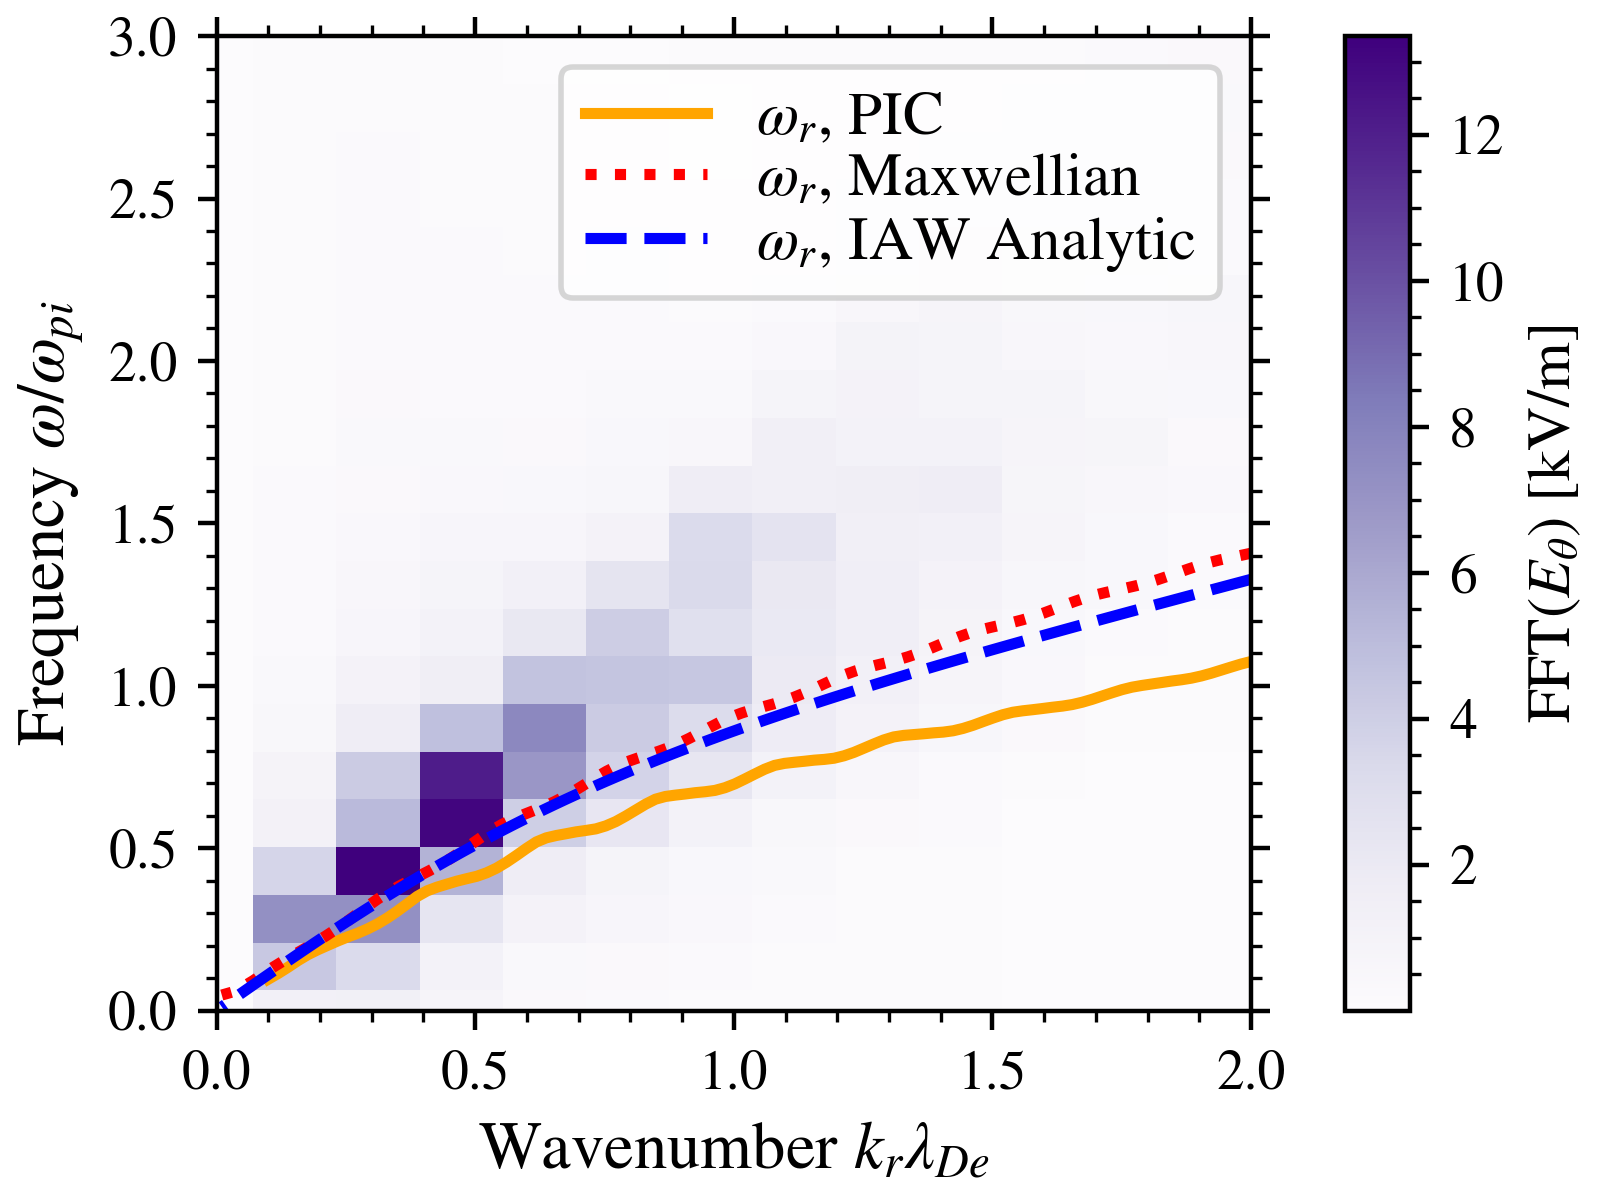
\includegraphics[width=\defaultwidth]{compe_fft_theo.png}
      \caption{Comparison of (purple image) the \acs{2D} \acs{FFT} of the azimuthal electric field $(E_{\theta})$ computed between  $t=0.6$ and $t=1.2\,\micro\second$ and averaged over the radial direction with the following dispersion relation\string: (orange solid) \acs{ECDI} general \acs{DR} obtained with the \acs{PIC} VDFs at $t=0.8\,\micro\second$; (dotted red) \acs{ECDI} \acs{DR} obtained with the Maxwellian hypothesis; and (dotted blue) \acs{IAW} \acs{DR} using the analytic expression \cref{eq-MIAW}.   }
      \label{fig-DR_and_fft}
    \end{figure}
    
    From \Cref{fig-DR_and_fft}, we can see that the instability observed in the \ac{PIC} simulation does follow the \ac{ECDI} \ac{DR} with a very good correspondence.
    However, the differences between the three \ac{DR} are not significant, compared to the resolution of the \ac{2D} \ac{FFT}.
    On top of that, the \ac{IAW} \ac{DR} returns almost the same values than that of the \ac{ECDI} \ac{DR}, as the resonances are no more present.
    Therefore we will use the \ac{IAW} \ac{DR} in the next section.
    
  \FloatBarrier
  \subsection{Resolution of the ion acoustic wave dispersion relation} \label{subsec-VDFIAW}
  
    We have seen in the previous \cref{subsec-ECDIPIC} that the full \ac{ECDI} dispersion relation is not needed, but can instead be approximated by the \ac{IAW} \citep{lafleur2018,janhunen2018,taccogna2019}.
    The \ac{IAW} relation can be solved with several hypotheses (see \cref{sec-geneDR} for more details)
    \begin{enumerate}
      \item Simplified analytical values,
      \item Maxwellian electrons, cold ion ($\Ti = 0\,\volt$),
      \item Maxwellian electrons and ions ($\Ti > 0\,\volt$),
      \item Non-Maxwellian electrons, Maxwellian ions ($\Ti > 0\,\volt$),
      \item Non-Maxwellian electrons and ions.
    \end{enumerate}
    
    In the following, we will use all these cases and compare them to the \ac{PIC} simulation results.
    We want to obtain the temporal evolution of the solution.
    In practice, we will only follow the evolution of the most growing wave.
    In order to find the most growing wave, we solve the dispersion relation for different values of $k$.
    Over all of the solutions obtained, we select the one corresponding to the maximum value of $\gamma$.
    We use 200 points between $k_{\theta}\lde=0.02 $ and $k_{\theta}\lde= 2$.
    \Cref{fig-Example_of_DR_IAW} illustrates how we select this dominant mode for one specific simulation time used for three different cases.
    We can see the maximum of the growing rate, and its frequency.
    
    \begin{figure}[hbt]
      \centering
      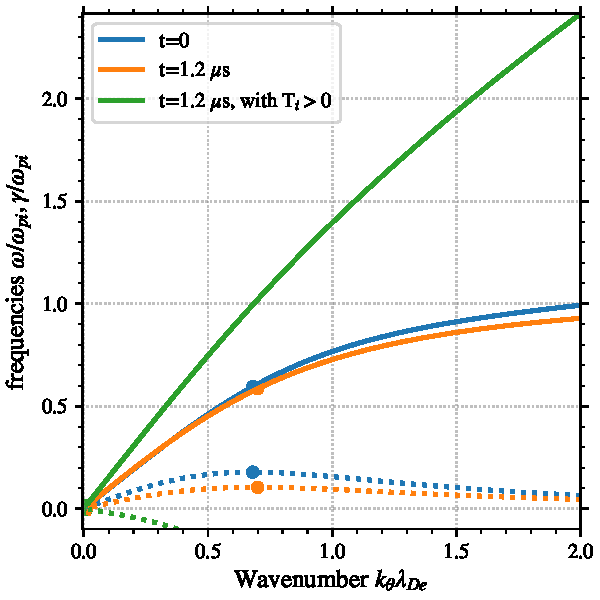
\includegraphics[width=4.5in]{Example_of_DR_IAW.pdf}
      \caption{Illustration of the \acs{IAW} dispersion relation obtained at two different time ($t=0$ and $t=1.2\,\micro\second$), (solid line) the wave frequency $\omega$, and (dotted line) the growth rate $\gamma$, using the hypothesis of Maxwellian distribution functions for both electrons and ions. The electron temperature measured in the simulation is always used, but the ion temperature is only used once. The most growing solution is marked with a circle on the growth rate and the frequency.}
      \label{fig-Example_of_DR_IAW}
    \end{figure}
    
    
    This process is repeated for the whole duration of the simulation.
    The velocity distribution functions, when used, are obtained from the \ac{PIC} simulation the same way as in \cref{subsec-VDFpic}.
    \Cref{fig-time_wave} shows the temporal evolution of the three characteristics of the most growing wave\string: the growth rate $\gamma$, the azimuthal wavenumber $k$ and the frequency $\omega$.
    \begin{figure}[hbt]
      \centering
      % 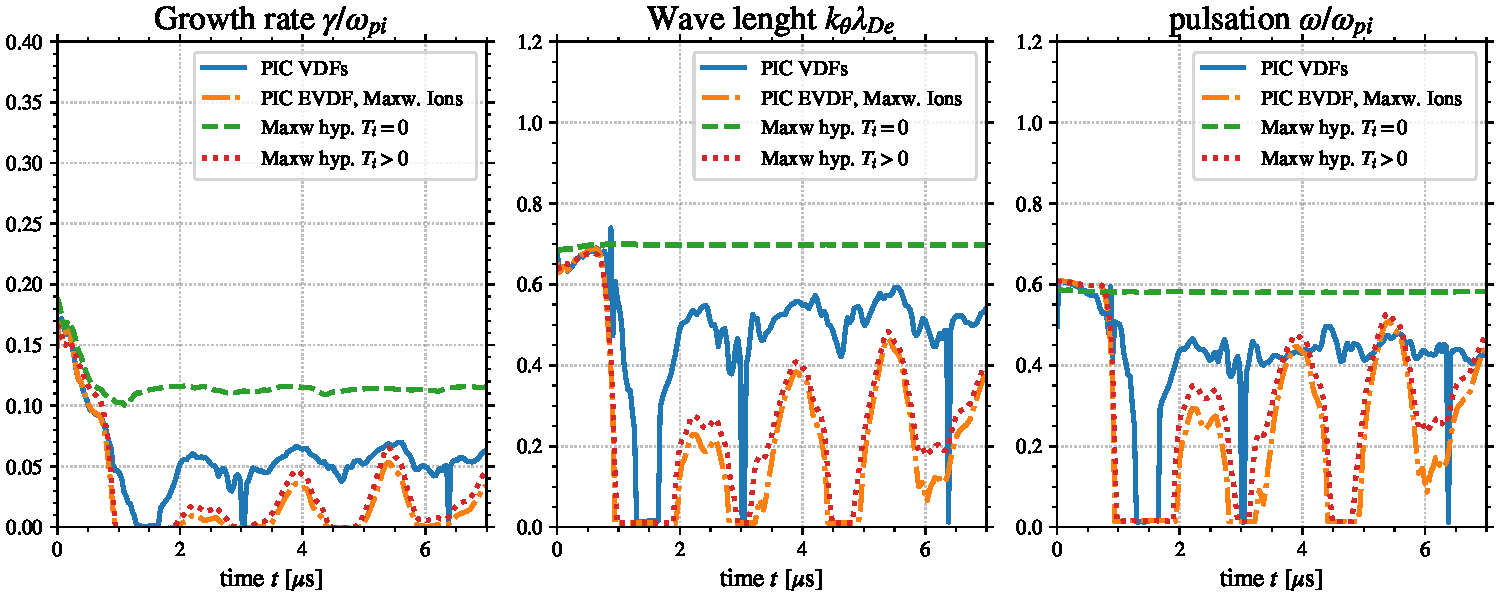
\includegraphics[width=\textwidth]{GrowthRate_time_evolution_250_ter.pdf}
      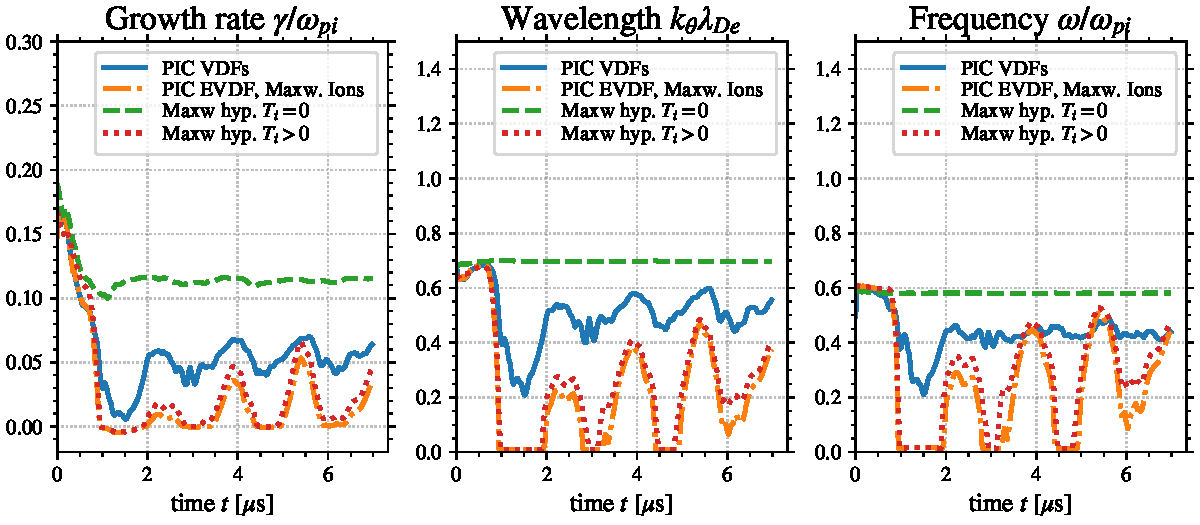
\includegraphics[width=\textwidth]{GrowthRate_time_evolution_250_notinverted.pdf}  %inverted ion velocity as a correction, to look like Lefleur... :/
      \caption{Temporal evolution of the growth rate $\gamma$, the azimuthal wavenumber $k$ and the frequency $\omega$ for the most growing wave, obtained with several hypotheses on the dispersion relation. See text for more details. }
      \label{fig-time_wave}
    \end{figure}
    
    Three different behaviors are observed depending on the hypotheses used.
    First, the solution of the dispersion relation with Maxwellian electrons and cold ions (dashed green line in \cref{fig-time_wave}) presents a solution of $\omega$ and $k$ constant in time, and very close to the analytic values, being $k_{\theta}\lde = 1/\sqrt{2}$ and $\omega_r = \opi/\sqrt{3}$.
    However, it also presents a constant growth rate.
    
    Secondly, we observe that the solutions assuming Maxwellian ions of non-zero temperature are relatively similar for both the Maxwellian electrons  (dotted red line) and using the electron velocity distribution function measured in the \ac{PIC} simulation (dash-dotted orange line).
    In these cases, the growth rate decreases regularly to zero.
    Interestingly, the periods during which the growth rate is zero (firstly between $t=1\,\micro\second$ and $t=2\,\micro\second$, then around $t=3\,\micro\second$ and so on) correspond precisely to the periods during which the wave energy density decreases in \cref{fig-tempITcrit}.
    With the Maxwellian hypothesis, the decrease of the growth rate is only be due to the ion temperature, which corresponds to ion Landau damping.
    However, we must note that the value of the ion temperature $\Ti$ is mainly due to the population of ions trapped, as seen in \cref{subsec-VDFpic}.
    
    To finish with, we solve the \ac{IAW} dispersion relation without any hypothesis on the velocity distribution functions, by using the VDF measured in the PIC simulations (blue solid line in  \cref{fig-time_wave}).
    In this case, the beginning ($t < 1 \,\micro\second$) is quite similar to the other results.
    Then for $t > 1 \,\micro\second$, the growth rate oscillates slightly around a mean value that is below the solution with cold ions, but above the result with warm ions.
    In order to determine which solution is the closest from the observation, we estimate the growth rate in the \ac{PIC} simulation with the wave equation
    \begin{equation} \label{eq-wequationbis}
      \deriv{W_{\rm PIC}}{t} + \div (\vect{u_i} W_{\rm PIC}) = 2 \gamma_{\rm PIC} W_{\rm PIC}
    \end{equation}
    with $W_{\rm PIC} = \sigma_{E_{\theta}}^2 \epsilon_0/2$ the electrostatic wave energy measured in the \ac{PIC} simulation.
    The spatial derivative can been approximated across the axial simulation direction by
    \begin{equation} \label{eq-}
      \div (\vect{u_i} W_{\rm PIC}) = \frac{ W_{\rm PIC} \viout}{L_z},
    \end{equation}
    with $\viout$ the ion outlet velocity 
    \begin{equation} \label{eq-vout}
      \viout = \sqrt{\frac{2 e U_z}{m_i}},
    \end{equation}
    with $U_z = E_z L_z$ the total potential difference in the axial direction.
    Therefore, the growth rate measured in the \ac{PIC} simulation is
    \begin{equation} \label{eq-picgrowthrate}
      \gamma_{\rm PIC} = \frac{ \partial_t W_{\rm PIC} }{W_{\rm PIC}}  +\frac{ \viout}{2 L_z}.
    \end{equation}
    \Cref{fig-pic_growth_rate} shows the temporal evolution of the growth rate of the most growing mode (similar to the left panel of \cref{fig-time_wave}) obtained with the relation dispersion, and $\gamma_{\rm PIC}$ the growth rate measured in the \ac{PIC} simulation using \cref{eq-picgrowthrate}.
    The value of $\gamma_{\rm PIC}$ is noisy, so we average it using a Gaussian kernel of standard deviation $\tau = 12\,\nano\second$.
    \begin{figure}[hbtp]
      \centering
      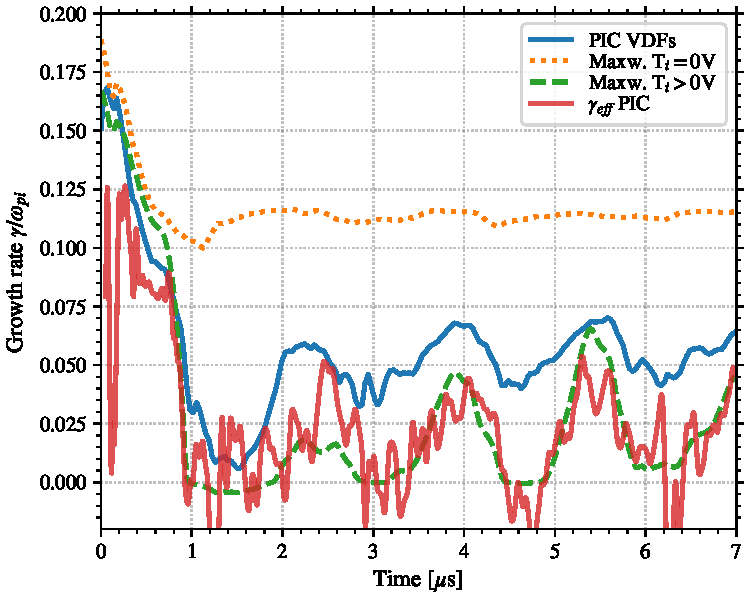
\includegraphics[width=\defaultwidth]{GrowthRate_time_evolution_onlygamma.pdf}
      \caption{Temporal evolution of the growth rate}
      \label{fig-pic_growth_rate}
    \end{figure}
    \inlinenote{Continue the legend}
    
    We see in \cref{fig-pic_growth_rate} that $\gamma_{\rm PIC}$, the growth rate measured in the simulation, follows the expected trend with an initial phase ($t<1\,\micro\second$) of growth, and then the oscillations with growing and damping phases.
    The values of $\gamma_{\rm PIC}$ are closer to the growth rate obtained with the Maxwellian hypothesis and a non-zero ion temperature (label "Maxw, $\Ti>0$" in \cref{fig-pic_growth_rate}), compared to the values obtained with the \ac{PIC} VDFs or with cold ions (label "Maxw, $\Ti=0$").
      %It is also in contrast with \citet{lafleur2018}, where the authors obtained a non-zero growth rate in an axial-azimuthal geometry.
      
      
    % \vspace{1em}
    % 
    % Up to now, there is non apparent explanation to the dependency  observed between the numerical resolution of the \ac{DR} and the results of the \ac{PIC} simulation.
    % It could be due to an error in the numerical algorithm, on both on the theory and in the implementation.
    % Concerning the theory, we have seen in \cref{sec-DR-solver} that the numerical algorithm used to compute the plasma dispersion function $\tilde{Z}$ proposed by \citet{xie2013} does not return a good result for certain argument complex values.
    % In addition, the truncation of the number of Fourier bases at $N=64$, which works well with a Maxwellian distribution, could generate a significant error when using distribution function far from a Maxwellian.
    % In our specific case, the ion population is composed of a majority of cold Maxwellian ions and a small number of high energetic trapped ions.
    % It is possible that this kind of distribution function is not well taken into account by the current algorithm.
    % 
    % Concerning the implementation of the algorithm, we tried to test and validate the code as much as we could, with systematic comparisons to analytic values.
    % But the presence of an error is always possible, that was not observed on the analytic functions.
    % A common practice to validate a simulation code when no theoretical solution can be used to compare to is to use a Benchmark \citep{turner2013}.
    % As a dispersion relation solver for general distributions would benefit the whole plasma physics community, developing such a benchmark that would compare the solution of independent implementations of the same algorithm, or different algorithm, seems very interesting.
    
  \FloatBarrier